\chapter{Redes Neuronales Artificiales}\label{cap:red_neuronal_tradicional}

En la actualidad, el término Red Neuronal Artificial (del inglés Artificial Neural Network, ANN) se ha vuelto tan popular y prácticamente igual de utilizado que el término IA, llegando a tratarlos casi como sinónimos. Nada más lejos de la realidad, nos remontamos a la década de los 40, cuando Alan Turing plantea un sistema que posteriormente sería desarrollado por Warren McCulloch y Walter Pitts, asentando así las bases de lo que hoy conocemos como IA, concretamente, en la rama del aprendizaje automático (del inglés Machine Learning, ML). Estos sistemas de computación están basados en el funcionamiento de las redes neuronales biológicas, es decir, el cerebro humano; intentan abstraer el complejo funcionamiento interno y centrarse en cómo nuestro cerebro procesa la información \cite{rna_fundamentos__hilera_2021}.

Nuestro cerebro es una compleja red de pequeños núcleos, llamados neuronas que están conectadas entre sí mediante brazos llamados axones. Estas se encargan de procesar la información que captamos del entorno mediante nuestros sentidos y nos permiten aprender en base a la experiencia y la exposición. Imaginemos a un niño pequeño que intenta aprender a diferenciar entre un círculo y un cuadrado. Cuando ve estas formas por primera vez, sus sentidos (vista, principalmente) captan la información visual, que es procesada en distintas regiones del cerebro como la corteza visual, encargada de interpretar patrones y características del entorno. A medida que el niño observa repetidamente estas figuras y recibe estímulos externos (como alguien que le dice “esto es un círculo”), su cerebro comienza a establecer conexiones entre lo que ve y lo que aprende. Estas conexiones ocurren entre neuronas, y cuanto más se repite la experiencia, más fuerte se vuelve la sinapsis entre ellas: este es el fundamento del aprendizaje. Además, la memoria del niño funciona de forma distribuida; puede recordar inmediatamente lo que ha aprendido (memoria a corto plazo), pero con la repetición y el uso frecuente, esa información se consolida y pasa a la memoria a largo plazo. Este proceso inspira a las redes neuronales artificiales, que intentan imitar cómo los humanos procesan información sensorial, aprenden mediante la repetición ajustando la “fuerza” de sus conexiones, y almacenan conocimiento de forma gradual y jerárquica.

Si bien es cierto que las redes neuronales no son tan complejas como sus homólogas biológicas, también poseen una estructura interna cuyo estudio es realmente importante. A grandes rasgos, podemos diferenciar tres factores importantes en la definición de una RNA: su arquitectura, es decir, la conexión entre sus neuronas, es decir, cómo están agrupadas y qué formas tienen de procesar la información; el algoritmo de aprendizaje utilizado, que definirá la forma en la que se calculan los pesos de las conexiones; y las funciones de activación, que permitirán introducir no linealidad en el modelo y decidir si una neurona se activa o no ante ciertos estímulos \cite{nn_fundamentals__thakur_2021}. La arquitectura de modelos es una subárea de la IA que se encarga del estudio del funcionamiento y la eficacia de la configuración de un modelo en función del conjunto de datos. Gracias a su desarrollo, podemos saber qué estructuras y configuraciones son mejores para ciertos tipos de problemas.

Siguiendo el ejemplo del niño pequeño que aprende a diferenciar formas, en el mundo de la IA existen problemas o conjuntos de datos que han sido ampliamente utilizados para verificar y testear el desarrollo de modelos. A lo largo del trabajo hablaremos sobre diferentes tipos de algoritmos y configuraciones, por lo que será necesario implicar a un sujeto de pruebas para ilustrar y comparar el rendimiento de cada enfoque. En concreto, el conjunto de datos será MNIST, un conjunto clásico y accesible que cuenta con un total de 70.000 imágenes de dígitos escritos a mano. Habiendo servido durante años como punto de partida en el desarrollo y evaluación de modelos de reconocimiento visual, este conjunto nos permitirá simular un proceso de aprendizaje progresivo en el que podamos observar cómo los distintos modelos son capaces de identificar patrones, adaptarse a la información y mejorar su precisión con la experiencia \cite{yolo_docs__2024}.

\section{Arquitectura de una Red Neuronal}\label{sec:arquitectura_rna}

Conceptualmente, una RNA está formada por unidades, llamadas neuronas, interconectadas y organizadas en lo que se denominan capas. Cada neurona se encarga de procesar desde una hasta múltiples señales de entrada, mediante la combinación de dos operaciones básicas: una combinación lineal ponderada de las entradas, y la aplicación de una función de activación no lineal. El resultado se transmite a las neuronas de la capa siguiente, de forma que la información siempre fluye unidireccionalmente desde la capa de entrada hasta la de salida. Por ejemplo, al procesar una imagen (representada como un vector de números) en la primera capa, cada unidad recibe una parte de la información de entrada, la procesa y entrega su resultado a la siguiente, así sucesivamente hasta que llegamos a la última capa y, por tanto, a la salida de la red. Combinando estos tratamientos, podemos lograr que una red sencilla sea capaz de, en primer lugar, detectar bordes; luego, que las capas intermedias los combinen para reconocer formas; y finalmente, que la última capa genere una clasificación final. Esto es, a rasgos generales, la estructura de una RNA \cite{neurocomputing__hecht_nielsen_1998}.

\begin{figure}[h]
	\centering
	\begin{tikzpicture}[colsep/.style={right=30mm of #1}]
		% layers
		\node (L1) at (0,0) {};
		\node[colsep=L1] (L2) {};
		\node[colsep=L2] (L3) {};

		\node[above=20mm of L1]{Entradas};
		\node[above=20mm of L2]{Capa oculta};
		\node[above=20mm of L3]{Salidas};

		\def\rio{1.2} % row steps inputs/outputs
		\def\rh{0.9} % row steps hidden

		% inputs
		\foreach \i in {1,...,3} {
			\node[neuron] (I\i) at ($(L1)+(0,{(2-\i)*\rio})$) {$x_{\i}$};
		}
		% hidden
		\foreach \i in {1,...,4} {
			\node[neuron] (H\i) at ($(L2)+(0,{(2.5-\i)*\rh})$) {$a_{\i}$};
		}
		% outputs
		\foreach \i in {1,...,2} {
			\node[neuron] (O\i) at ($(L3)+(0,{(1.5-\i)*\rio})$) {$y_{\i}$};
		}

		% edges
		\foreach \i in {1,...,3} \foreach \j in {1,...,4} \draw[edge] (I\i) -- (H\j);
		\foreach \j in {1,...,4} \foreach \k in {1,...,2} \draw[edge] (H\j) -- (O\k);

	\end{tikzpicture}
	\caption{Red neuronal totalmente conectada (3–4–2).}
	\label{fig:red_neuronal_simple}
\end{figure}


\subsection{Las capas}

Como hemos mencionado, existen diferentes tipos de capa: la capa de entrada, es la interfaz de la red, recibe datos vectorizados y los transmite al resto de capas \cite{intro_rna__rivera_2005}; las capas ocultas, que realizan transformaciones no lineales mediante matrices de pesos y funciones de activación; la capa de salida, encargada de traducir y codificar el resultado de la red a un formato interpretable en el contexto del problema. El aprendizaje ocurre mediante el ajuste dinámico de los pesos de las conexiones durante el entrenamiento, permitiendo a las capas ocultas extraer características jerárquicamente más abstractas de los datos \cite{neurocomputing__hecht_nielsen_1998}.

La cantidad de neuronas de una capa oculta puede variar dependiendo del caso, pero no existe ningún método que nos permita determinar su número óptimo. Numerosos estudios destacan que solo la experimentación durante el entrenamiento permite aproximar cuántas unidades se requieren para una tarea específica. Además, en ciertos escenarios complejos puede requerirse la incorporación de múltiples niveles ocultos, aunque en la mayoría de las aplicaciones, dos capas ocultas suelen ser suficientes \cite{rna_fundamentos__hilera_2021}.

\subsection{La neurona}

La neurona es la unidad computacional básica, es en ella donde se relizan todas las operaciones para determinar la salida de la red. Su estructura consta de tres componentes: canales de entrada, núcleo y canales de salida.

Los canales de entrada son las interfaces por las que la neurona recibe las señales $x_1, x_2, \dots, x_n.$ Normalmente, se representa con un vector cuyas posiciones tienen un peso $w_i$ asociado (la memoria de la red), con lo que se determina qué entradas son más importantes. Luego, el núcleo, en el que se aplican dos funciones: la función de combinación (de las entradas y sus pesos), y la función de activación, que aplica una transformación no lineal. Por último, el canal de salida por el que transmite el resultado a las neuronas de la capa siguiente, sirviendo de entrada para nuevos cálculos \cite{intro_rna__rivera_2005}.

Los pesos $w_i$ constituyen la "memoria" de la red y se optimizan durante el entrenamiento para minimizar errores. Aunque la arquitectura es fija, la capacidad de aprendizaje proviene de la adaptación de estos parámetros con cada iteración \cite{dl_python__chollet_2021}.

\begin{figure}[h]
	\centering
	\begin{tikzpicture}
		\node (L1) at (0,0) {};
		\node[right=25mm of L1] (L2) {};
		\node[right=25mm of L2] (L3) {};

		\node[above=15mm of L1]{Entradas};
		\node[above=15mm of L2]{Neurona $i$};
		\node[above=15mm of L3]{Salida};

		% inputs
		\foreach \i in {1,...,3} \node (I\i) at ($(L1) + (0,2-\i)$) {$x_{\i}$};
		% neurona central
		\node[neuron] (N) at (L2) {$a(z_{i})$};
		% output
		\node (O) at (L3) {$y_{i}$};

		\foreach \i in {1,...,3} \draw[edge weight] (I\i) -- node {$w_{\i}$} (N);
		\draw[edge] (N) -- (O);

	\end{tikzpicture}
	\caption{Diagrama funcionamiento neurona simple.}
	\label{fig:diagrama_neurona_simple}
\end{figure}

\subsubsection{Función de Combinación}\label{f_combinacion}

La función de combinación transforma las entradas $\vec{x} = \left [ x_1, x_2, ..., x_n\right ]^T$ utilizando sus pesos asociados $\vec{w} =  \left [ w_1, w_2, ..., w_n\right ]$, se representa con la operación punto ($\cdot$). Su forma estándar es la suma ponderada:

\begin{equation}\label{f_combinacion:suma_ponderada}
z = \vec{w}\cdot\vec{x} = \sum_{i=1}^{n}(w_i \cdot x_i)
\end{equation}

Existen diferentes modificaciones de esta función, como aplicar funciones de agregación como el $\max(z)$ o el $\min(z)$, o combinaciones booleanas como la conjunción $\bigwedge_i(w_i \wedge x_i)$ o la disyunción $\bigvee_i(w_i \vee x_i)$, todo dependerá del contorno del problema. Sin embargo, suma ponderada \eqref{f_combinacion:suma_ponderada} es ampliamente utilizada por su diferenciabilidad\footnote{La diferenciabilidad es un concepto fundamental en el cálculo infinitesimal y la matemática en general. Se refiere a la propiedad de una función de poder ser derivada en un punto específico \cite{analisis_matematico__gordon_1995}.}, propiedad esencial para el entrenamiento mediante el descenso del gradiente \cite{dl_python__chollet_2021}.

\subsubsection{Función de Activación}\label{f_activacion}

El propósito de una función de activación es el de introducir \textbf{no linealidad} en el modelo, permitiendo que la red aprenda relaciones complejas en los datos. Sin funciones de activación, una red neuronal sería equivalente a una simple regresión lineal (combinación lineal de todas las capas $L_T = L_1 + L_2 + \dots + L_n$), incapaz de resolver problemas complejos como el reconocimiento de imágenes o el procesamiento del lenguaje natural \cite{dl_python__chollet_2021, dl_fundamentos__casas_roma_2020}.

Su nombre proviene de la capacidad que tiene para decidir si la neurona \textit{se activa} o no. Como se puede observar en la figura \ref{fig:diagrama_neurona_simple}, toma el valor $z$ de salida de la combinación \eqref{f_combinacion:suma_ponderada} y le aplica una operación matemática no lineal $a = \sigma(z)$, donde $\sigma$ representa la función de activación. Decimos que la neurona se activa cuando supera el umbral de la función de activación, y consecuentemente, decimos que no se activa cuando no supera dicho umbral. Por ejemplo, en un problema binario, en el que las salidas deben ser 0 o 1, podemos utilizar \ref{f_activacion:umbral} como función de activación \cite{nn_dl__michael_nielsen_2015}, donde $th$ es el umbral de activación.

\begin{equation}\label{f_activacion:umbral}
\left \{
    \begin{array}{ccc}
    0 & si & \vec{w}\cdot\vec{x} \leq th \\
    1 & si & \vec{w}\cdot\vec{x} > th \\
    \end{array}
\right .
\end{equation}

Debido a la búsqueda de una notación más simplificada y cómoda, el umbral de activación se suele desplazar al primer término de la desigualdad y reemplazarlo por lo que se conoce como el sesgo de la neurona ($b \equiv -th$), tal y como en \ref{f_activacion:sesgo} \cite{nn_dl__michael_nielsen_2015}.

\begin{equation}\label{f_activacion:sesgo}
\left \{
    \begin{array}{ccc}
    0 & si & \vec{w}\cdot\vec{x} + b\leq 0 \\
    1 & si & \vec{w}\cdot\vec{x} + b > 0 \\
    \end{array}
\right .
\end{equation}

Esta modificación permite expresar el umbral como si fuese otra entrada más a la neurona con $1$ como peso asociado. Simplificando nuestra función de combinación a \ref{f_combinacion:sesgo}.

\begin{equation}\label{f_combinacion:sesgo}
z = \vec{w} \cdot \vec{x} + b
\end{equation}

Los sesgos son un factor clave para la activación de una neurona o no. Cuanto mayor sea su valor más sencillo será para una neurona activarse, mientras que si toma un valor muy negativo, puede llegar a ser muy difícil que esa neurona se active \cite{nn_dl__michael_nielsen_2015}. Tanto los pesos $w_i$ y como los sesgos $b$ se ajustan iterativamente durante el entrenamiento. Este proceso permite a la red priorizar entradas relevantes asignando pesos altos a características discriminativas, suprimir ruido atenuando señales irrelevantes (pesos cercanos a cero) y modelar compensaciones, ya que el sesgo actúa como umbral de activación base.


\paragraph{Perceptrón}

Existen diferentes tipos de funciones de activación y elegiremos una u otra en función de el contorno del problema y el tipo de dato que vayamos a utilizar. El ejemplo más simple para definir la activación de una neurona es la función escalón (utilizada en \ref{f_activacion:sesgo}), utilizada en neuronas binarias. Cuando la combinación de entradas de la neurona es mayor al umbral, la activación es 1; si es menor, es 0 (aunque el rango puede cambiar, por ejemplo, a $\{-1,1\}$) \cite{rna_fundamentos__hilera_2021}.

\begin{equation}\label{f_activacion:escalon}
   \sigma(z) = \left \{
        \begin{array}{ccc}
            0 & si & z \leq 0 \\
            1 & si & z > 0
        \end{array}
   \right .
\end{equation}

Una neurona que aplique la suma ponderada, como función de combinación, y la función escalón, como función de activación, se denomina \textbf{perceptrón}. Esta arquitectura fue inventada y propuesta por Frank Rosenblatt en 1958 \cite{perceptron__rosenblatt_1958} y a día de hoy se utiliza como base de estudio y comprensión del funcionamiento de las redes neuronales. Sin embargo, el perceptrón clásico presenta una limitación para el aprendizaje automático: su función escalón produce salidas binarias (0 o 1), lo que imposibilita realizar ajustes graduales en los pesos durante el entrenamiento \cite{nn_dl__michael_nielsen_2015}, es decir, un pequeño ajuste en los pesos puede ocasionar un gran desajuste en la salida de la red.

Si modificamos ligeramente un peso o sesgo en un perceptrón, su salida puede cambiar abruptamente (de 0 a 1). Esta discontinuidad propaga cambios caóticos en redes multicapa, haciendo inviable optimizar los parámetros de forma sistemática \cite{nn_dl__michael_nielsen_2015}. Para resolver esto, se desarrollaron funciones de activación alternativas con dos propiedades clave:

\begin{enumerate}
    \item Diferenciabilidad: permitir calcular gradientes suaves para ajustar pesos mediante descenso de gradiente.
    \item No linealidad suave: transformar la suma ponderada ($z$) de manera progresiva, no abrupta.
\end{enumerate}

\paragraph{Sigmoide}

Le neurona sigmoide\footnote{Es común que, en la literatura técnica, las neuronas se nombren según la función de activación que utilizan.} fue la primera en resolver las limitaciones del perceptrón ya que \ref{f_activacion:sigmoide} genera salidas continuas, a la vez que pequeños cambios $\Delta w_i$ en sus pesos producen cambios proporcionales $\Delta a$ en la salida, permitiendo a la red aprender mediante correcciones incrementales (importante para la retropropagación de la red) \cite{nn_dl__michael_nielsen_2015}.

\begin{equation}\label{f_activacion:sigmoide}
    \sigma(z) = \frac{1}{1 + e^{-z}}
\end{equation}

A simple vista, la neurona sigmoide parece muy diferente del perceptrón. Sin embargo, si realizamos un pequeño análisis algebráico veremos que la función sigmoide no es más que aplicar un filtro de suavizado a la función escalón. Supongamos que $z \equiv \vec{w}\cdot\vec{x} + b$ es un número positivo muy grande. Entonces $e^{-z} \approx 0$, por tanto, $\sigma(z) = 1$. Es decir, si $z$ es un número positivo grande, la función de activación de la neurona será aproximadamente $1$, de forma similar al perceptrón. Por otro lado, si $z$ es un número negativo, entonces $e^{-z} \rightarrow \infty$, y $\sigma(z) \approx 0$. De forma que, cuando $z$ es muy negativo, la función de activación tenderá a valer $0$, aproximando el funcionamiento de un perceptrón \cite{nn_dl__michael_nielsen_2015}.

Si bien es cierto que el uso de la sigmoide permitió aplicar técnicas como el aprendizaje mediante gradientes, su diseño plantea ciertas lagunas. Al mapear valores extremos de $z$ (positivos o negativos) a regiones cercanas a $0$ o $1$, la derivada de la función se vuelve casi nula. Este fenómeno se conoce como desvanecimiento del gradiente (\textit{vanishing gradient} del inglés) y dificulta el ajuste de pesos en capas profundas, ya que los gradiente se atenuan exponencialmente (van desapareciendo, como el nombre indica) durante la retropropagación \cite{dl_fundamentos__casas_roma_2020}. Además, plantea otro problema relacionado con el intervalo $(0,1)$ de salida de la función, haciendo que todas sus neuronas generen valores positivos, ralentizando la convergencia en el entrenamiento. Actualmente, este tipo de neurona se utiliza sobre todo en modelos de clasificación binaria \cite{dl_python__chollet_2021}.

\paragraph{ReLU} \label{sec:relu}

La unidad lineal rectificada (ReLU, por sus siglas en inlgés) es una función de activación ampliamente adoptada en redes neuronales profundas debido a su simplicidad y eficacia. Definida por la ecuación \ref{f_activacion:relu}, ReLU transforma la salida de la función de combinación $z$ aplicando una no linealidad con umbral en cero:

\begin{equation}\label{f_activacion:relu}
    \sigma(z) = \max(0, z) = (z)^+
\end{equation}

A diferencia de la sigmoide, ReLU preserva la linealidad para valores positivos de $z$, lo que facilita el flujo del gradiente durante el entrenamiento y mitiga el problema de desaparición del gradiente en redes profundas. Además, su cálculo es computacionalmente eficiente, ya que solo require comparar $z$ con cero, evitando operaciones exponenciales costosas como en la sigmoide. A rasgos generales, las redes basadas en ReLU mejoran el rendimiento consistentemente en comparación a las redes basadas en funciones de activación sigmoide \cite{dl_python__chollet_2021}.

Sin embargo, el uso de las ReLU también conlleva riesgos. Cuando una neurona recibe constantemente entradas negativas $(z \leq 0)$, su salida y gradiente se acaban anulando, y como consecuencia, sus pesos también. Este problema, bautizado como \textbf{neuronas muertas}, puede inutilizar una sección de la red. Existen variantes como la \textit{Leaky ReLU} o la \textit{Parametric ReLU} que intentan mitigar estos riesgos \cite{dl__goodfellow_2016}.

\section{Entrenamiento}\label{sec:entrenamiento_rn}

A lo largo de la primera sección hemos desglosado superficialmente los componentes principales de una red neuronal tradicional, desde la arquitectura de las neuronas hasta el papel de las funciones de activación. Sin embargo, estos elementos sólo constituyen el esqueleto de datos de las redes.

El proceso de entrenamiento es el mecanismo por el cual un modelo es capaz de asimilar las diferentes características de un conjunto de datos, aprendiendo así, a reconocer patrones complejos, generalizar relaciones entre entradas y salidas, o incluso, a realizar predicciones en datos nunca vistos. Para llegar a esto, el modelo deberá pasar por diferentes etapas en su entrenamiento con el fin de optimizar sus parámetros internos: el conjunto de pesos $W^i$ y el sesgo $b$ de cada neurona \cite{dl_fundamentos__casas_roma_2020}.

Interiorizar estos conceptos nos permite no solo entender cómo las redes neuronales aprenden, sino que también asienta las bases para diseñar arquitecturas más eficaces y diagnosticar problemas comunes como el sobreajuste, o el estancamiento en mínimos locales.

\paragraph{Preparación de los Datos}

A la hora de entrenar entra en juego un factor casi tan importante como el propio modelo, el conjunto de datos de entrenamiento. Al igual que los atletas necesitan una dieta equilibrada y que potencie ciertas vitaminas para exprimir sus capacidades físicas en las competiciones, los modelos necesitan que el conjunto de datos que se utilice para entrenarlos capture la esencia del problema que se quiere resolver.

Generalmente, en la etapa de entrenamiento nos ayudaremos de tres conjuntos de datos: el conjunto de entrenamiento, una colección de datos que el modelo iterará para aprender las características y relaciones del problema; el conjunto de validación, que nos ayudará a evaluar el modelo tras cada entrenamiento y a ajustar sus hiperparámetros\footnote{Características configurables de una red neuronal tales como el número o el tamaño de las capas, las funciones de activación, el método de inicialización de pesos, etc. Es decir, todo aquello que no se modifica automáticamente a lo largo del aprendizaje de la red \cite{dl_python__chollet_2021, dl_fundamentos__casas_roma_2020}.}; y el conjunto de pruebas, la colección de datos que nos permitirá verificar el rendimiento y la eficacia del entrenamiento al final del proceso.

\begin{figure}[h]
	\centering
	\includegraphics[width=0.8\linewidth]{figures/ejemplos/preparacion_datos_mnist.png}
	\caption{Preparación del conjunto de datos MNIST en los subconjuntos de entrenamiento, validación y pruebas.}
	\label{fig:preparcion_datos_mnist}
\end{figure}

Normalmente, la separación de datos en sus diferentes conjuntos suele realizarse aleatoriamente, aunque, se intenta mantener la proporción $20$-$80$ o $30$-$70$ para los subconjuntos de pruebas y entrenamiento, respectivamente. Una vez separados los subconjuntos, podríamos utilizarlos sin problema. No obstante, existen diferentes metodologías o prácticas para dividir los datos de manera que los preparemos para el modelo. Entre los más conocidos está el \textit{$K$-fold Cross Validation} \cite{dl_python__chollet_2021, dl_fundamentos__casas_roma_2020}.

\textbf{K-fold Cross Validation}. Consiste en segmentar el conjunto de datos en $K$ subconjuntos o \textit{folds} de tamaño similar. En cada iteración \(k=1,\dots,K\), se entrena el modelo con \(K-1\) folds y se valida con el fold restante. Al finalizar, se promedian las métricas para obtener una estimación más robusta del rendimiento y reducir la varianza asociada a una única partición entrenamiento-pruebas.

\begin{figure}[h!]
	\centering
	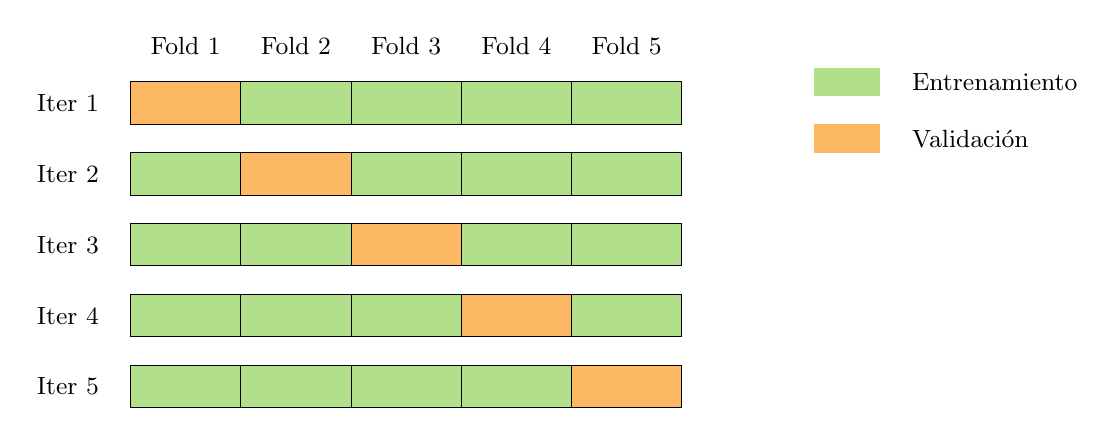
\begin{tikzpicture}[x=1.4cm,y=0.9cm,font=\small]
		%%% Colores
		\definecolor{traincolor}{RGB}{178,223,138} % verde claro
		\definecolor{valcolor}{RGB}{253,184,99}    % naranja claro
		\def\K{5}
		\def\cellh{0.6}

		%%% Cabeceras de columnas (folds)
		\foreach \j [evaluate=\j as \lab using int(\j+1)] in {0,...,4} {
			\node[anchor=south] at (\j+0.5, 0.25) {Fold \lab};
		}

		%%% Cuadrícula: filas = iteraciones, columnas = folds
		\foreach \row [evaluate=\row as \it using int(\row+1)] in {0,...,4} {
			% Etiqueta de fila (iteración/fold de validación)
			\node[anchor=east] at (-0.2, -\row-\cellh/2) {Iter \it};

			\foreach \col in {0,...,4} {
				% Validación: columna que coincide con la fila
				\ifnum\col=\row
				\fill[valcolor] (\col, -\row) rectangle ++(1,-\cellh);
				\else
				\fill[traincolor] (\col, -\row) rectangle ++(1,-\cellh);
				\fi
				\draw (\col, -\row) rectangle ++(1,-\cellh);
			}
		}

		%%% Leyenda
		\begin{scope}[shift={(6.2, -0.2)}]
			\fill[traincolor] (0,0) rectangle ++(0.6,0.4);
			\node[anchor=west] at (0.8,0.2) {Entrenamiento};

			\fill[valcolor] (0,-0.8) rectangle ++(0.6,0.4);
			\node[anchor=west] at (0.8,-0.6) {Validación};
		\end{scope}
	\end{tikzpicture}
	\caption{Esquema de \emph{K-fold Cross Validation} con \(K=5\): en cada iteración, un fold distinto (naranja) se usa para validación y los restantes (verde) para entrenamiento.}
	\label{fig:kfold_cross_validation_ejemplo}
\end{figure}



\subsection{Retropropagación}\label{sec:retropropagacion}

La magia del aprendizaje automático se fundamenta en un algoritmo conocido como retropropagación (\textit{backpropagation}, en inglés). Esta técnica consiste en utilizar una función de coste al final de la red que mida la discrepancia entre el valor inferido y el real. Posteriormente, propagaremos el error desde el final hasta la primera capa de la red, actualizando sistemáticamente todos los parámetros internos que intervienen en la predicción, de forma que en la siguiente iteración hacia adelante (\textit{forward}, en inglés) se reduzca la magnitud del error \cite{dl_fundamentos__casas_roma_2020}.

Existen diferentes funciones de pérdida, todas relacionan la salida esperada $y$ con la predicción del modelo $\hat{y}$. En este trabajo nos centraremos en una de las más básicas y utilizadas en la literatura: el error cuadrático.

\begin{align}\label{f_error:cuadratico}
    E = \frac{1}{2}(\hat{y}-y)^2
\end{align}

A lo largo de la retropropagación, utilizaremos el error calculado por funciones como esta para poder actualizar todos los parámetros. Sin embargo, no todos ellos se actualizarán de la misma forma. Tenemos que ser capaces de discernir qué neuronas estuvieron más implicadas en la decisión de la red, de forma que la magnitud del cambio sea proporcional a la responsabilidad. En el mundo matemático, las herramientas utilizadas para medir la variación de un parámetro respecto de otro es la \textbf{derivada}. Esta es la base del algoritmo utilizado por antonomasia en el entrenamiento de modelos de aprendizaje automático: el descenso del gradiente.

\paragraph{Descenso del Gradiente} \label{sec:descenso_gradiente}

Imaginemos que somos una persona con los ojos vendados en mitad de una montaña. Si quisiéramos descenderla, bastaría con, iterativamente, dar pequeños pasitos en dirección a donde la pendiente sea menor. Básicamente, este es el razonamiento detrás del descenso del gradiente. Siendo la función del error una función continua, podemos calcular la derivada respecto de uno de sus parámetros para estudiar la pendiente y hallar mínimos locales. Eso, en resumen, es lo que hace nuestra red para aprender.

Hagamos un ejemplo con un sistema en $2D$. Supongamos el final de una iteración de nuestro modelo, que nuestra función de coste es el error cuadrático y el valor esperado en la inferencia es 0, nuestra función de coste quedaría $f(x) = \frac{1}{2}(x)^2$. En este punto, siendo la red, tendríamos que calcular cómo varía el error en función del valor de nuestros parámetros. La derivada de nuestra función de coste es $f'(x) = x$. Todo esto se puede escribir en python de forma muy simple utilizando la sintaxis de las expresiones lambda.

\begin{lstlisting}[language=Python,label=code:descenso_grad_2d_1]
	import numpy as np
	f_error = lambda x: 1/2 * (x)**2
	df_error = lambda x: x
\end{lstlisting}

Luego, para representar nuestra función de coste vamos a generar un array de valores que nos permitan ver la gráfica del error centrada. Como la expresión del coste define una parábola con vértice en el $0$, crearemos un vector de $1000$ valores entre el $-1$ y el $1$. Además, seleccionaremos un punto aleatorio de este vector, ya que la inicialización de parámetros es aleatoria.

\begin{lstlisting}[language=Python,label=code:descenso_grad_2d_2]
	data = np.linspace(-1, 1, num=1000)
	rnd_x = np.random.choice(data, 1)
\end{lstlisting}

Es aquí donde entrea en juego nuestro algoritmo de optimización. Vamos a iterar sobre esta función de coste, para cada paso vamos a calcular hacia dónde tiene que moverse nuestro punto para minimizar el error. Para ello, utilizaremos la derivada junto con un factor de cambio que decidimos nosotros. Con él, controlaremos la magnitud del cambio sobre el punto, más tarde ahondaremos en este concepto.

\begin{lstlisting}[language=Python,label=code:descenso_grad_2d_3]
	fig, ax = plt.subplots()
	ax.plot(data, f_error(data), label='f_error', color='black')
	ax.scatter(rnd_x, f_error(rnd_x), color='red', label='inicio')

	change_rate = 0.01
	for _ in range(250):
		slope = df_error(rnd_x)
		rnd_x = rnd_x - slope * change_rate
		step = ax.scatter(rnd_x, f_error(rnd_x), marker='.', color='blue')

	ax.scatter(rnd_x, f_error(rnd_x), color='green', label='final')
\end{lstlisting}

Todas estas iteraciones, nos dan como resultado el descenso de la función de coste definida, bajando su pendiente.

\begin{figure}[hb]
	\centering
	\includegraphics[width=0.6\linewidth]{figures/ejemplos/gradient_descent_2d.png}
	\caption{Descenso del gradiente para el error cuadrático. Cada paso acerca $x$ al mínimo global ($x=0$).}
	\label{fig:descenso_gradiente_2d}
\end{figure}

Aunque es simplista, este ejemplo nos ayuda a hacernos una idea de cómo funciona por dentro la actualización de los parámetros. Claro que, en una red, trabajamos a nivel multidimensional, donde los parámetros son tensores, contenedores $n$-dimensionales. En estos casos la notación se vuelve un poco más verbosa, ya que tenemos que emplear el \textbf{gradiente} \cite{dl_python__chollet_2021}.

Por definición, el gradiente de la función de coste $\nabla E$ es un vector que apunta hacia la dirección de máximo aumento del error. Su magnitud indica la tasa de cambio en esa dirección, es decir, cuanto mayor sea, mayor variación habrá. Por tanto, si buscamos $-\nabla C$, nuestro vector gradiente estará apuntando hacia donde el valor del error se minimiza, que, de hecho, es lo que buscamos para el aprendizaje de la red. Si modificamos un poco el código anterior, podemos realizar un ejemplo en $3D$. En este caso, usando dos vectores, $\vec{x}$ e $\vec{y}$, la función del error la expresaremos con lo que en la literatura se denomina \textit{one-hot encoding}. Esta notación consiste en relacionar las clases de predicción con las posiciones de un vector. Aquellas clases que son correctas se marcan con el valor $1$ en la posición correspondiente, el resto a $0$. Traduciendo el caso anterior, en el que el valor esperado era un $0$. El error se calcularía como $f(x) = \frac{1}{2} ((x-1)^2 + y^2)$.

\begin{lstlisting}[language=Python,label=code:descenso_grad_3d_1]
	f_error = lambda x, y: 1/2 * ((x - 1)**2 + y**2)
	dfdx_error = lambda x: x - 1
	dfdy_error = lambda y: y

	data = np.linspace(-10,10,1000)
	x, y = np.meshgrid(data, data)
	rnd_x = np.random.choice(data, 1)
	rnd_y = np.random.choice(data, 1)

	fig, ax = plt.subplots()
	contour = ax.contourf(x, y, f_error(x,y), levels=10)
	ax.scatter(rnd_x, rnd_y, color='red', label='inicio')

	change_rate = 0.01
	for _ in range(250):
		slope_x = dfdx_error(rnd_x)
		slope_y = dfdy_error(rnd_y)
		rnd_x = rnd_x - slope_x * change_rate
		rnd_y = rnd_y - slope_y * change_rate
		step = ax.scatter(rnd_x, rnd_y, color='blue', marker='.')

	ax.scatter(rnd_x, rnd_y, color='green', label='final')
\end{lstlisting}

Ajustando el resto del código a este formato obtendríamos una representación tridimensional del descenso del gradiente de nuestra función de coste, desde un punto elegido aleatoriamente (punto rojo), paso a paso, hasta el mínimo (global) del error (punto verde).

\begin{figure}[htb]
	\centering
	\includegraphics[width=0.7\linewidth]{figures/ejemplos/gradient_descent_3d.png}
	\caption{Descenso del gradiente en 3D del error cuadrático. Cada paso acerca $(x,y)$ al mínimo global $f(x,y) = 0$.}
	\label{fig:descenso_gradiente_3d}
\end{figure}


A grandes rasgos, en cada iteración el algoritmo de retropropagación se encargará de distribuir ese error a lo largo de todas las conexiones de la red, calculando en cada nodo cómo varía la salida de la red respecto a ese parámetro buscando que la función del error se minimize. Es decir, acabamos de convertir el aprendizaje de la red neuronal en un problema de optimización \cite{dl__goodfellow_2016}.


\paragraph{Actualización de los Parámetros} \label{sec:actualizacion_parametros}

Como hemos visto a lo largo de la implementación del descenso del gradiente, una de las etapas más importantes es la actualización de los parámetros. Gracias a esto, el modelo es capaz de aprender por cuenta propia, ajustándose automáticamente para ser capaz de inferir con precisión. Comúnmente, a la hora de actualizar los parámetros se utiliza lo que se denomina la \textbf{regla delta} en la literatura. Esto no es más que una formalidad para referirse al incremento o el decremento del valor de los parámetros.

\begin{equation}\label{regla_delta}
	\Delta x = \eta \frac{dE}{dx} \rightarrow x = x - \frac{dE}{dx}
\end{equation}

En esta expresión redescubrimos un factor muy importante en la actualización de los pesos. Previamente, en el descenso del gradiente, regulamos la magnitud del cambio calculado en la derivada con un ratio de cambio. Este ratio de cambio expresa la "velocidad" a la que queremos que nuestro modelo aprenda. En la literatura se conoce como \textbf{tasa de aprendizaje} y en función de su valor, podemos provocar que el modelo aprenda tan lento que nunca llegue a adquirir todas las características del problema, pudiendo incluso estancarse en mínimos locales; o por el contrario, si la tasa es muy grande, el modelo difícilmente encuentrará el mínimo en el error. La elección de la tasa de aprendizaje determina la velocidad y la estabilidad del entrenamiento. Un valor óptimo permitirá a la red descender suavemente hacia configuraciones de error mínimo \cite{dl_python__chollet_2021, dl_fundamentos__casas_roma_2020, dl__goodfellow_2016}.

Con este ejemplo hemos podido comprender mejor cómo funciona la optimización de parámetros en una red monocapa. Pero ¿qué ocurre cuando tenemos más de una capa? El descenso del gradiente es una técnica que nos permite saber cómo serán las variaciones del error en función de los parámetros de la capa directamente anterior a la salida. Es decir, al utilizar redes multicapa sólo podríamos afinar los parámetros de las neuronas de la penúltima capa de la red. Es aquí donde, la regla de la cadena, entra en juego, permitiéndonos calcular fácilmente el gradiente de arquitecturas complejas \cite{dl_python__chollet_2021}.


\paragraph{La Regla de la Cadena} \label{sec:regla_cadena}

Recapitulando un poco, hemos logrado adquirir las herramientas necesarias para calcular cómo corregir el error de predicción de nuestro modelo. Sin embargo, nuestros modelos son complejas estructuras de cálculo, pareciese que el cálculo final del error no tuviese nada que ver con aquella entrada en la primera capa. ¿O sí? Cierto es que nuestros modelos son complejas redes de nodos interconectados, donde cada salida depende de una serie de operaciones intermedias. Para poder ajustar los parámetros desde la última capa hasta la primera necesitamos una manera sistemática de propagar esas derivadas hacia atrás a lo largo de la red.

Aquí entra en juego la regla de la cadena, una herramienta matemática que nos permite descomponer la derivada de una función en términos de derivadas parciales más simples. En otras palabras, la regla de la cadena actúa como un mecanismo de transmisión: el gradiente fluye desde la salida hasta las entradas atravesando cada operación que conecta ambos extremos. En la literatura, se utilizan una serie de expresiones matemáticas \footnote{Consultar \ref{anexo:retropropagacion}.}. No obstante, este trabajo pretende arrojar un pequeño haz de luz e intuición. Por tanto, nos centraremos en la idea sobre la que se construyeron los modelos matemáticos.

Para entenderlo de forma intuitiva, consideremos un ejemplo sencillo $f(x,y,z) = (x+y)z$, que podemos simplificar todavía más como $q=(x+y)$ y $f=qz$. En la figura \ref{fig:forward_pass_diagrama} se muestra el grafo que desglosa las operaciones para $f(2,3,4)$.

\begin{figure}[ht]
	\centering
	\includegraphics[width=0.6\linewidth]{figures/ejemplos/forward_diagram.png}
	\caption{Diagrama de la función $f(x,y,z)=(x+y)z$, para $(x,y,z)=(2,3,4)$.}
	\label{fig:forward_pass_diagrama}
\end{figure}

Este diagrama, en esencia, representa lo que ocurre en una red al hacer \textit{forward}. Ahora, queremos calcular la responsabilidad de cada entrada dentro de la operación para, en caso de querer corregir los valores, saber la magnitud con la que actualizaremos cada uno. Es decir, tenemos que calcular las derivadas parciales de $f$ respecto de cada entrada: $\frac{\partial f}{\partial x}$, $\frac{\partial f}{\partial y}$ y $\frac{\partial f}{\partial z}$. Para ello, aplicaremos la regla de la cadena de las derivadas. Esta nos dice que podemos descomponer la derivada de una función en términos más simples. En nuestro caso, utilizaremos la expresión $f=qz$ como paso intermedio para calcular las derivadas parciales respecto de $x$ e $y$.

\begin{equation}
	\frac{\partial f}{\partial x} = \frac{\partial f}{\partial q} \frac{\partial q}{\partial x} \qquad
	\frac{\partial f}{\partial y} = \frac{\partial f}{\partial q} \frac{\partial q}{\partial y}
\end{equation}

Para $z$ no tenemos el mismo inconveniente, ya que en la expresión $f=qz$ existe una relación directa entre la función y la variable. Ahora sí, podemos calcular paso a paso las derivadas parciales por la regla de la cadena:

\begin{figure}[h!]
	\centering
	\includegraphics[width=0.6\linewidth]{figures/ejemplos/backward_diagram.png}
	\label{fig:backward_diagrama}
	\caption{Diagrama de regla de la cadena de la función $f(x,y,z)=(x+y)z$, para $(x,y,z)=(2,3,1)$.}
\end{figure}

En resumen, la retropropagación permite trasladar la información del error desde la salida de la red hasta sus capas más profundas mediante la aplicación sistemática de la regla de la cadena. Gracias a este mecanismo, cada parámetro recibe una corrección proporcional a su contribución en la predicción final. Este procedimiento convierte a la retropropagación en el motor principal del aprendizaje en redes neuronales: a través de sucesivas iteraciones de propagación hacia adelante, cálculo de error y propagación hacia atrás, el modelo ajusta sus parámetros internos hasta capturar patrones útiles en los datos.

De este modo, lo que en apariencia es un entramado complejo de nodos y conexiones, se convierte en un sistema entrenable y optimizable. Esta combinación de cálculo diferencial y optimización numérica constituye la base matemática sobre la que se sustentan las arquitecturas modernas de aprendizaje profundo.


\subsection{Generalización y Regularización}

Hasta el momento, hemos abordado el aprendizaje de una red neuronal como un problema de optimización, con el propósito principal de entrenar modelos que no solo funcionen bien con los datos utilizados durante el entrenamiento, sino que también sean capaces de realizar predicciones precisas en datos nuevos. Esta capacidad de desempeñarse correctamente en situaciones no vistas previamente se conoce como \textit{generalización} \cite{dl__goodfellow_2016}. En esencia, buscamos desarrollar modelos que identifiquen patrones útiles y aplicables a distintos contextos, evitando simplemente memorizar los ejemplos específicos del conjunto de entrenamiento.

\paragraph{Problemas comunes en el entrenamiento}
De acuerdo con \citeauthor{dl__goodfellow_2016}, la capacidad de un modelo para generalizar correctamente depende tanto de su habilidad para minimizar el error en los datos de entrenamiento como de su eficacia al enfrentarse a las diferencias entre los conjuntos de entrenamiento y prueba. En este contexto, se identifican principalmente los siguientes problemas:

\begin{itemize}
	\item \textbf{Sobreajuste}: ocurre cuando la red neuronal memoriza detalles irrelevantes del conjunto de entrenamiento en lugar de aprender patrones significativos. El resultado es un rendimiento deficiente en datos nuevos.
	\item \textbf{Subajuste}: aparece cuando el modelo es demasiado simple para capturar la complejidad de los datos, lo que impide alcanzar un buen desempeño incluso en el propio conjunto de entrenamiento.
	\item \textbf{Alta varianza y sesgo}: relacionados respectivamente con modelos excesivamente complejos (varianza elevada) o excesivamente simples (alto sesgo).
\end{itemize}

Para mitigar estas situaciones, existen diversas técnicas que actúan directamente sobre los parámetros del modelo durante el entrenamiento, conocidas como regularización, entre las más utilizadas se encuentran la L1 y L2, el dropout y la normalización de los batches.

\textbf{Regularización L1.} Consiste en añadir un término proporcional a la suma de los valores absolutos de los pesos en la función de pérdida:

\begin{equation}
	\mathcal{L}_{total} = \mathcal{L}_{original} + \lambda \sum_{i} |w_i|
	\label{eq:l1_reg}
\end{equation}

Este mecanismo promueve la \textit{esparsidad} en los parámetros, forzando a que muchos de ellos tomen valor cero. De este modo, el modelo tiende a ser más simple y puede realizar una selección implícita de características relevantes.

\textbf{Regularización L2.} También denominada \textit{weight decay}, esta técnica penaliza la magnitud cuadrática de los pesos:

\begin{equation}
	\mathcal{L}_{total} = \mathcal{L}_{original} + \lambda \sum_{i} w_i^2
	\label{eq:l2_reg}
\end{equation}

A diferencia de L1, no fuerza explícitamente pesos nulos, pero sí tiende a mantenerlos pequeños. Esto contribuye a estabilizar el entrenamiento y mejorar la capacidad de generalización al evitar que el modelo dependa en exceso de ciertos parámetros.

\textbf{Dropout.} Es una técnica estocástica que consiste en "desactivar" de forma aleatoria un subconjunto de neuronas durante cada paso del entrenamiento, el tamaño de ese subconjunto se suele configurar entre un $0.2$ y un $0.5$ del total de neuronas de la capa. De esta forma, la red no puede depender excesivamente de neuronas concretas y se ve obligada a explorar otros caminos dentro de la red, volviéndose más robusta. Cuando no se entrena, todas las neuronas se activan y sus salidas se escalan con el factor de dropout para compensar el efecto del entrenamiento \cite{dl_python__chollet_2021}.

\begin{figure}[h]
	\centering
	\begin{tikzpicture}[>=Latex, every node/.style={font=\small}]
		% Parámetros
		\def\nin{5}   % número de neuronas en la capa l
		\def\nout{4}  % número de neuronas en la capa l+1
		\def\dy{1.2}  % separación vertical entre neuronas
		\def\dx{4.0}  % separación horizontal entre capas

		% Capa 1 (entradas)
		\foreach \i in {1,...,\nin}{
			\node[circle, draw, minimum size=8mm] (I\i) at (0,-\i*\dy) {};
		}
		\node[above=2mm of I1] {Capa $l$};

		% Coordenada y del centro de la primera capa
		\pgfmathsetmacro{\yin}{-(\nin+1)/2 * \dy}

		% Coordenada y del centro de la segunda capa
		\pgfmathsetmacro{\yout}{-(\nout+1)/2 * \dy}

		% Capa 2 (salidas), centrada verticalmente respecto a la capa 1
		\foreach \j in {1,...,\nout}{
			\node[circle, draw, minimum size=8mm] (O\j) at (\dx,{\yin+\yout + \j*\dy}) {};
		}
		\node[above=8mm of O4] {Capa $l+1$};

		% Conexiones por defecto
		\foreach \i in {1,...,\nin}{
			\foreach \j in {1,...,\nout}{
				\draw[gray!60] (I\i) -- (O\j);
			}
		}

		% Resaltar dos neuronas apagadas en capa l
		\node[circle, draw, minimum size=8mm, fill=gray!30] at (I2.center) {};
		\node at (I2.center) {\textcolor{red}{\Large$\times$}};

		\node[circle, draw, minimum size=8mm, fill=gray!30] at (I4.center) {};
		\node at (I4.center) {\textcolor{red}{\Large$\times$}};

		% Dibujar conexiones activas más fuertes desde las otras neuronas
		\foreach \j in {1,...,\nout}{
			\draw[->, thick, blue] (I1) -- (O\j);
			\draw[->, thick, blue] (I3) -- (O\j);
			\draw[->, thick, blue] (I5) -- (O\j);
		}
	\end{tikzpicture}
	\caption{Ilustración del dropout: algunas neuronas (en gris con aspa) se desactivan de forma aleatoria durante el entrenamiento, forzando a la red a no depender de unidades específicas.}
	\label{fig:dropout}
\end{figure}



\textbf{Batch Normalization.} Aplica una transformación que mantiene la media de la salida a 0 y la desviación estándar a 1. No funciona igual durante el entrenamiento que durante la inferencia. Durante el entrenamiento, utiliza la media y la desviación estándar del batch para normalizar los datos de entrada. Durante las inferencias, el modelo utiliza un promedio móvil de la media y la desviación estándar de los batches que vió en el entrenamiento. Esta técnica, facilita la retropropagación de los gradientes del modelo, lo cual ayuda en modelos profundos \cite{dl__goodfellow_2016}.

En conjunto, estas técnicas permiten controlar la complejidad del modelo y mitigar el sobreajuste, contribuyendo a un mejor equilibrio entre rendimiento en entrenamiento y capacidad de generalización en datos no vistos.

\section{Limitaciones de las Redes Neuronales Tradicionales}\label{sec:limitaciones_rn}

Las redes neuronales densamente conectadas, aunque son efectivas en tareas de aprendizaje general, presentan desafíos al aplicarse a multidimensionales, como las imágenes.

Una de sus principales limitaciones es su incapacidad para aprovechar la estructura espacial. Por ejemplo, en imágenes, trata cada píxel como una entrada independiente, ignorando las relaciones de proximidad entre píxeles adyacentes, fundamental para identificar patrones locales como bordes, texturas o formas.

\begin{figure}[h]
	\centering
	\includegraphics[width=0.7\linewidth]{figures/ejemplos/imagen_a_red_neuronal.png}
	\caption{Aplanado de una imagen para servir de entrada a una red neuronal.}
	\label{fig:aplanado_imagen_red_neuronal}
\end{figure}

Adicionalmente, esta condición provoca lo que se conoce como \textit{redundancia en el aprendizaje de características}, donde cada neurona debe aprender pesos específicos para detectar una característica en una posición particular, como por ejemplo la neurona $a_{3}^{1}$ de la figura \ref{fig:aplanado_imagen_red_neuronal}, incluso si dicha característica ha aparecido en otra región de la imagen, limitando su generalización.

Por otra parte, intentar modelar problemas que involucren imágenes de gran
tamaño (por ej. 100x100 píxeles) puede convertirse en un reto de escalabilidad en el que los parámetros
crezcan exponencialmente. Una capa densa con 1000 neuronas requeriría millones
de pesos, lo que conlleva un alto coste computacional, riesgo de overfitting y
un alto consumo de memoria.

Con la intención de sobrepasar dichas limitaciones, las redes convolucionales introducen mecanismos específicos adaptados a datos visuales. Mediante operaciones de \textbf{convolución}, que aplican filtros locales que trabajan con \textit{ventanas} en la imagen, permitiendo al modelo preservar la estructura bidimensional de la entrada y aprender patrones espaciales jerárquicamente.

